\documentclass[xcolor=svgnames]{beamer}

% #### graphics and schemes
\usepackage{graphicx}
\graphicspath{{img/}}
\usepackage{tikz}
\usetikzlibrary{shapes,decorations,mindmap,trees}
\usepackage{array}
\usepackage{listings}
\usepackage{ccicons}

% #### theme
\useoutertheme{sidebar}
\useinnertheme{circles}
\usecolortheme{sidebartab}
\usecolortheme{seahorse}
\beamertemplatenavigationsymbolsempty

% #### colors
\usepackage{xcolor}

% #### layouts
\usepackage{multicol}
\usepackage[labelfont=footnotesize,textfont=scriptsize,bf]{caption}
\usepackage{subfig}

% #### math
\usepackage[squaren]{SIunits}

% #### fonts
\usepackage[utf8]{inputenc}
\usepackage[italian]{babel}
\usepackage[T1]{fontenc}
\usepackage{cmbright}
\usepackage{soul}
\usepackage{hyperref}
\urlstyle{same}
\usepackage{bbding}

% #### mainmatter
\title[Geodati e software liberi in archeologia]{OSM e GFOSS: geodati e software liberi\\in archeologia}
\author[Francesco \mbox{de Virgilio}]{Francesco de Virgilio \\ \texttt{\tiny francesco.devirgilio@fradeve.org}}
\date[GFOSSDay 2011]{GFOSS Day 2011\\\footnotesize{Nov 24--25, Foggia}}

%% ##### logo matter ####
\pgfdeclaremask{uniba}{uniba-logo}
\pgfdeclareimage[mask=uniba,width=2cm]{osm-logo}{../img/osm/osm-logo}
\logo{\vbox{\vskip0.1cm\hbox{\pgfuseimage{osm-logo}}}}


\begin{document}

	% #### automatically prints toc when section starts
	\AtBeginSection[]
		{
		\begin{frame}
			\frametitle{Sommario}
			\begin{multicols}{2}
				\tableofcontents[currentsection]
			\end{multicols}
		\end{frame}
		}

	{
	\usebackgroundtemplate{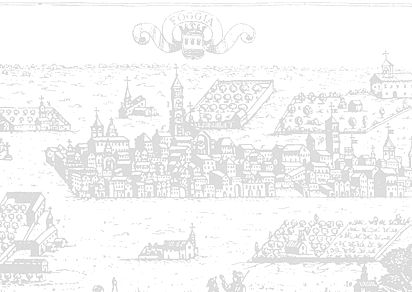
\includegraphics[width=1.5\paperwidth]{../img/osm/foggia_ancient2}}
	\begin{frame}
		\titlepage
	\end{frame}
	}

	% -----------------------------------------------------

	\begin{frame}{Benvenuti a Foggia}
		\centering
\includegraphics[width=0.8\textwidth]{../img/osm/proprietaria}
		\vfill
		\begin{center}
			\textit{Tutti i diritti sono riservati. Nessuna parte di questa edizione può essere riprodotta, memorizzata o trasmessa in alcuna forma e con alcun mezzo\ldots}
		\end{center}
	\end{frame}

	% -----------------------------------------------------

	\begin{frame}{Storia}
		\centering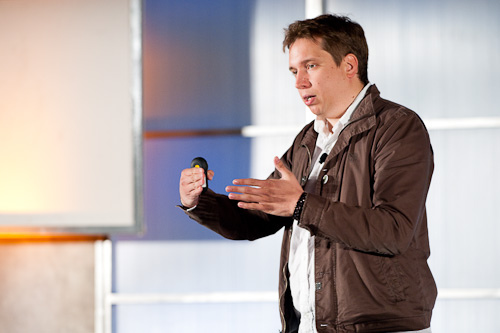
\includegraphics[width=0.8\textwidth]{../img/osm/steve}
		\begin{center}
			Steve Coast
		\end{center}
	\end{frame}

	% -----------------------------------------------------

	\begin{frame}{OpenStreetMap}
		\begin{block}{Cos'è?}
			OpenStreetMap è un progetto che punta a creare e fornire dati cartografici liberi e gratuiti a chiunque ne abbia bisogno; questi dati vengono usati per creare una mappa collaborativa del Pianeta.
		\end{block}
		\vfill
		\centering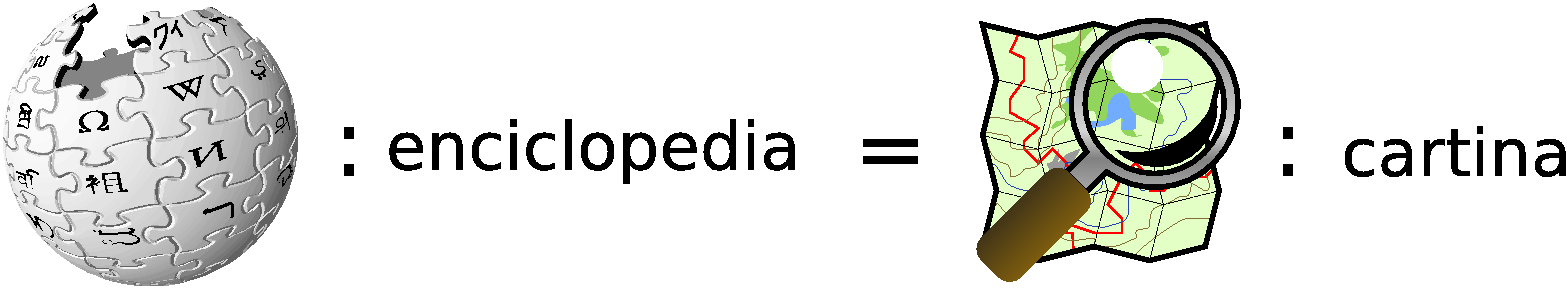
\includegraphics[width=0.8\textwidth]{../img/osm/osm-wiki}
	\end{frame}

	% -----------------------------------------------------

	\begin{frame}{Creatività!}
		Il progetto è stato lanciato perché la gran parte delle mappe che potresti pensare essere gratuite, hanno invece - oltre a frequenti errori - restrizioni legali o tecniche al loro uso, impedendo alle persone il loro uso per scopi produttivi, creativi ed altri.

		\begin{center}
			\fontsize{60}{70}\selectfont \ccShareAlike
		\end{center}
	\end{frame}

	% -----------------------------------------------------
	
	\begin{frame}{Geodati e PA -- \small{trova l'errore}}
		\centering\includegraphics[width=0.8\textwidth]{../img/osm/pa}\\
	\end{frame}

	% -----------------------------------------------------

	\begin{frame}
		\begin{columns}[c]
			\column{.4\textwidth}
				\begin{center}
					
\includegraphics[width=0.8\textwidth]{../img/osm/question}
				\end{center}
			\column{.6\textwidth}
				\huge Le carte che uso non sono già libere? Le trovo su internet\ldots
		\end{columns}
	\end{frame}

	% -----------------------------------------------------

	\begin{frame}
		\begin{center}
			\fontsize{50}{60}\selectfont No.
		\end{center}
	\end{frame}

	% -----------------------------------------------------

	\begin{frame}{È tutto chiuso}
		In generale, le mappe che si trovano su internet non sono libere, ma coperte da diritto d'autore, che ne limita o proibisce qualsiasi utilizzo non autorizzato; in questa situazione ricadono anche:

		\begin{itemize}
			\item Google Maps \footnotesize{(presto a pagamento?)}
			\item Tom Tom
			\item Garmin
		\end{itemize}

		Inoltre, le mappe protette da diritto d'autore:

		\begin{itemize}
			\item hanno errori fatti ad arte
			\item non rendono disponibili i dati sorgente
			\item non sono aggiornate / complete
			\item non si possono correggere
			\item non si possono rivendere / utilizzare per altri scopi
		\end{itemize}
	\end{frame}

	% -----------------------------------------------------

	\begin{frame}{Affidabilità [1]}
		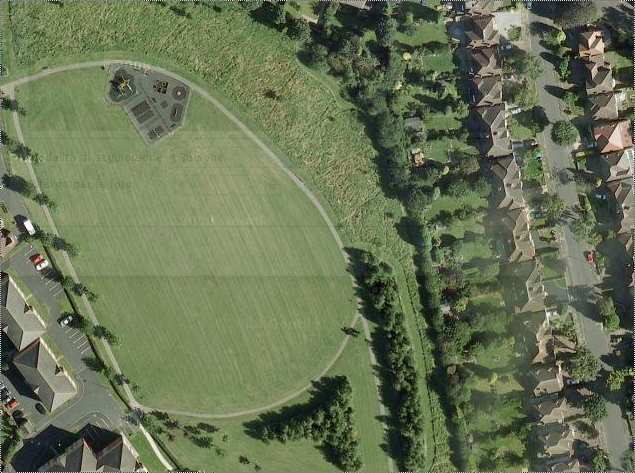
\includegraphics[width=0.51\textwidth]{../img/osm/err_1_1}
		\hfill
		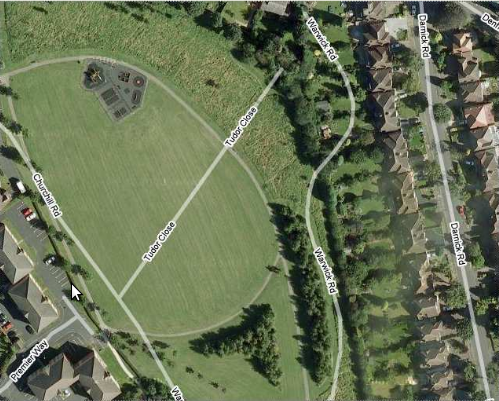
\includegraphics[width=0.477\textwidth]{../img/osm/err_1_2}
		\begin{center}
			Sutton coldfield, Regno Unito; Warvick Road non esiste!
		\end{center}
	\end{frame}

	% -----------------------------------------------------

	\begin{frame}{Affidabilità [2]}
		\begin{center}
			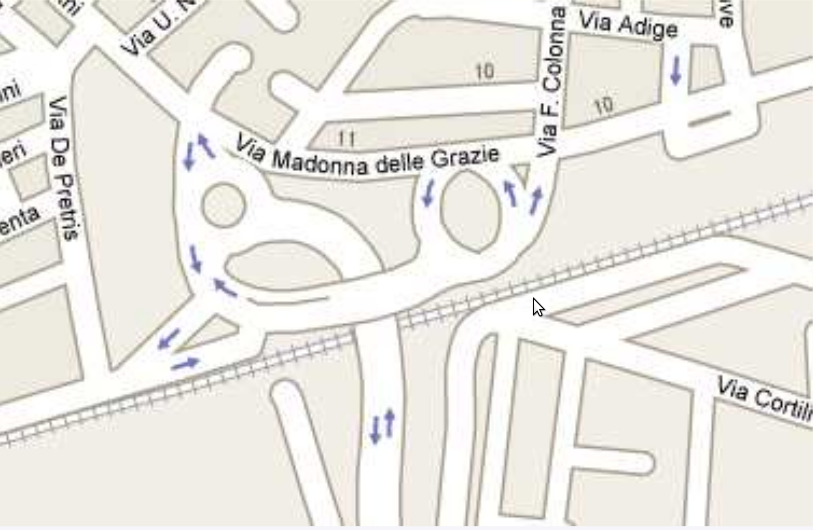
\includegraphics[width=0.8\textwidth]{../img/osm/err_2}
		\end{center}
		\begin{center}
			Terlizzi, \st{sovra} sotto--passaggio
		\end{center}
	\end{frame}

	% -----------------------------------------------------

	\begin{frame}{Affidabilità [3]}
		\begin{center}
			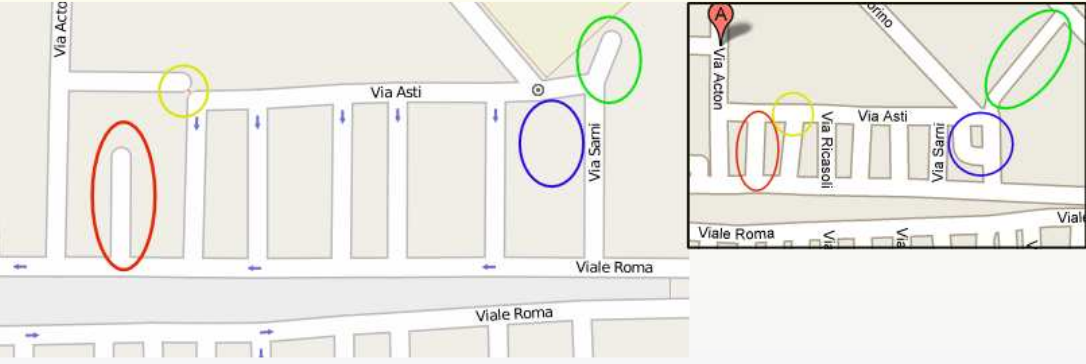
\includegraphics[width=1\textwidth]{../img/osm/err_3}
		\end{center}
		\begin{center}
			Terlizzi, 4 errori in 100 metri
		\end{center}
	\end{frame}

	% -----------------------------------------------------

	\begin{frame}
		\begin{columns}[c]
			\column{.4\textwidth}
				\begin{center}
					
\includegraphics[width=0.8\textwidth]{../img/osm/5_green}
				\end{center}
			\column{.6\textwidth}
				\Huge 5 semplici fasi
		\end{columns}
	\end{frame}

	% -----------------------------------------------------

	\begin{frame}{Partecipare ad OpenStreetMap}
		\begin{center}
			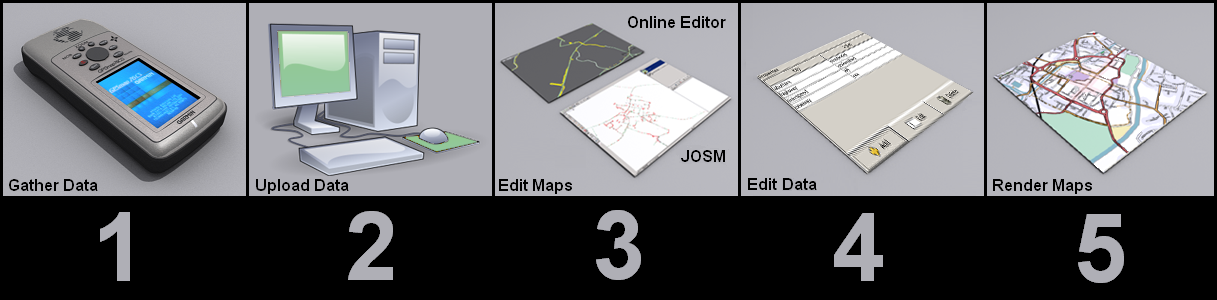
\includegraphics[width=1\textwidth]{../img/osm/sum}
			\vfill
			\huge \HandCuffRightUp~\url{www.openstreetmap.org}
		\end{center}
	\end{frame}

	% -----------------------------------------------------

	\begin{frame}{Raccogliere dati}{migliorando quanto fatto da altri}
		\begin{center}
			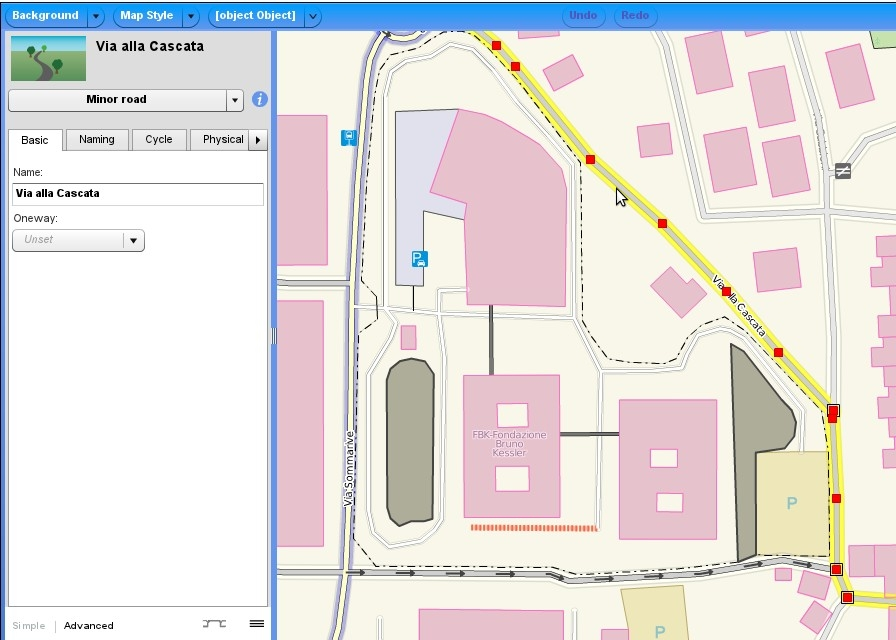
\includegraphics[width=1\textwidth]{../img/osm/potlatch}
		\end{center}
	\end{frame}

	% -----------------------------------------------------

	\begin{frame}{Raccogliere dati}{contribuendo a mappe tematiche}
		\begin{center}
			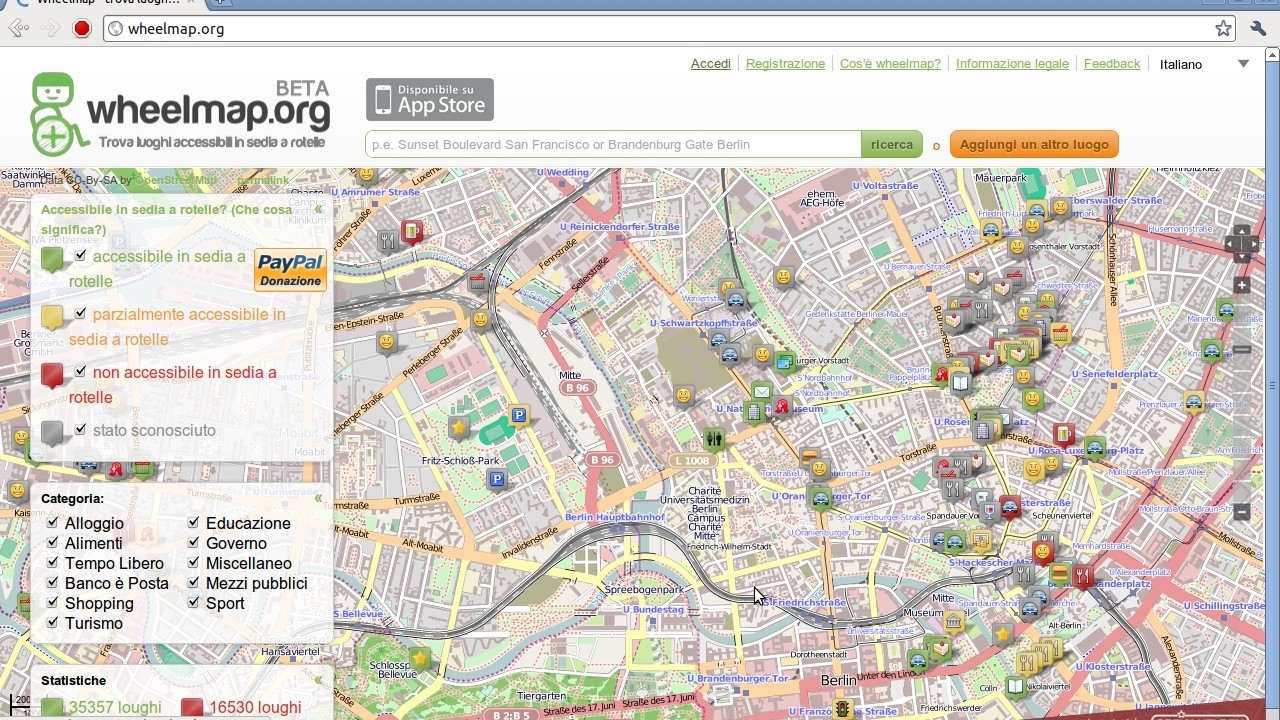
\includegraphics[width=1\textwidth]{../img/osm/wheel}
		\end{center}
	\end{frame}

	% -----------------------------------------------------

	\begin{frame}{Raccogliere dati}{ricalcando foto aeree}
		\begin{center}
			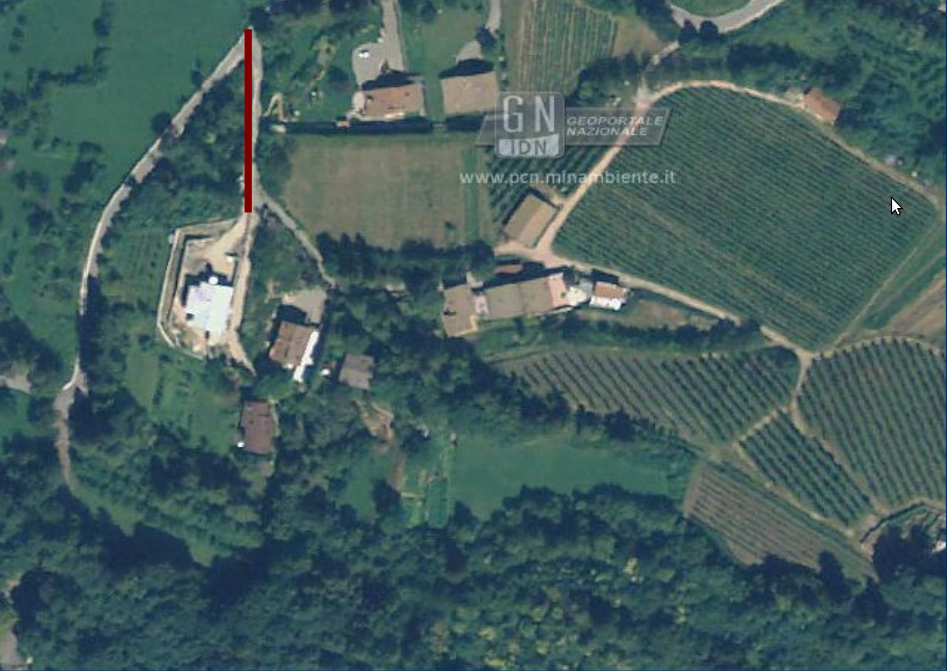
\includegraphics[width=0.9\textwidth]{../img/osm/orto}
		\end{center}
	\end{frame}

	% -----------------------------------------------------

	\begin{frame}{Raccogliere dati}{usando il GPS}
		\begin{center}
			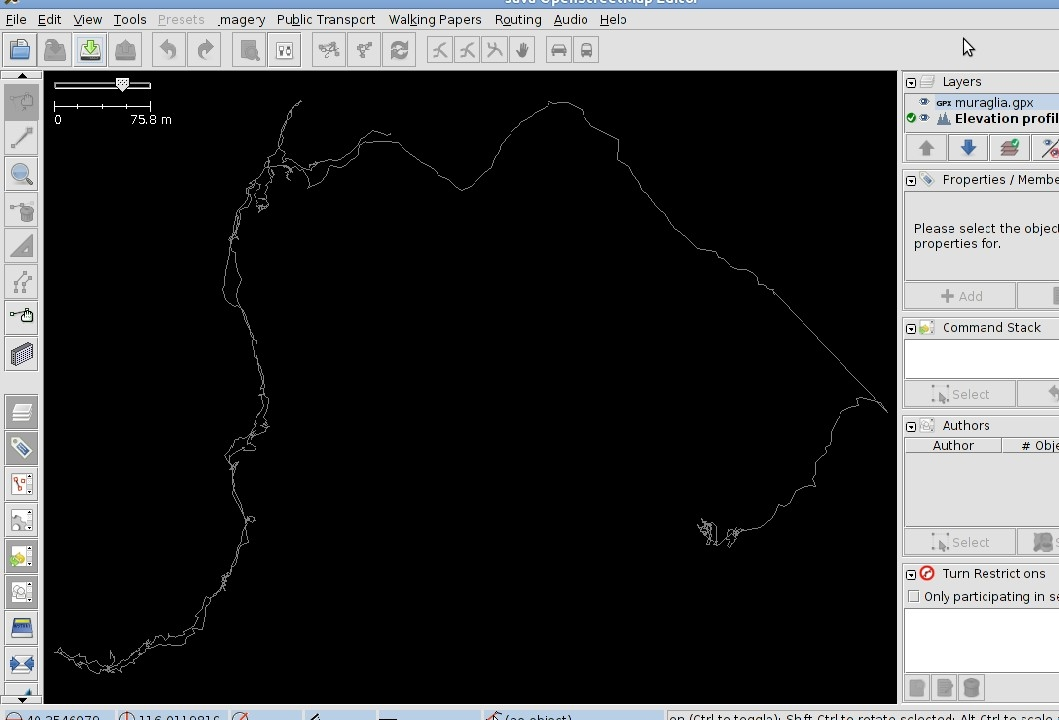
\includegraphics[width=0.95\textwidth]{../img/osm/gps}
		\end{center}
	\end{frame}

	% -----------------------------------------------------

	\begin{frame}{Raccogliere dati}{attraverso i \textit{walking papers}}
		\begin{center}
			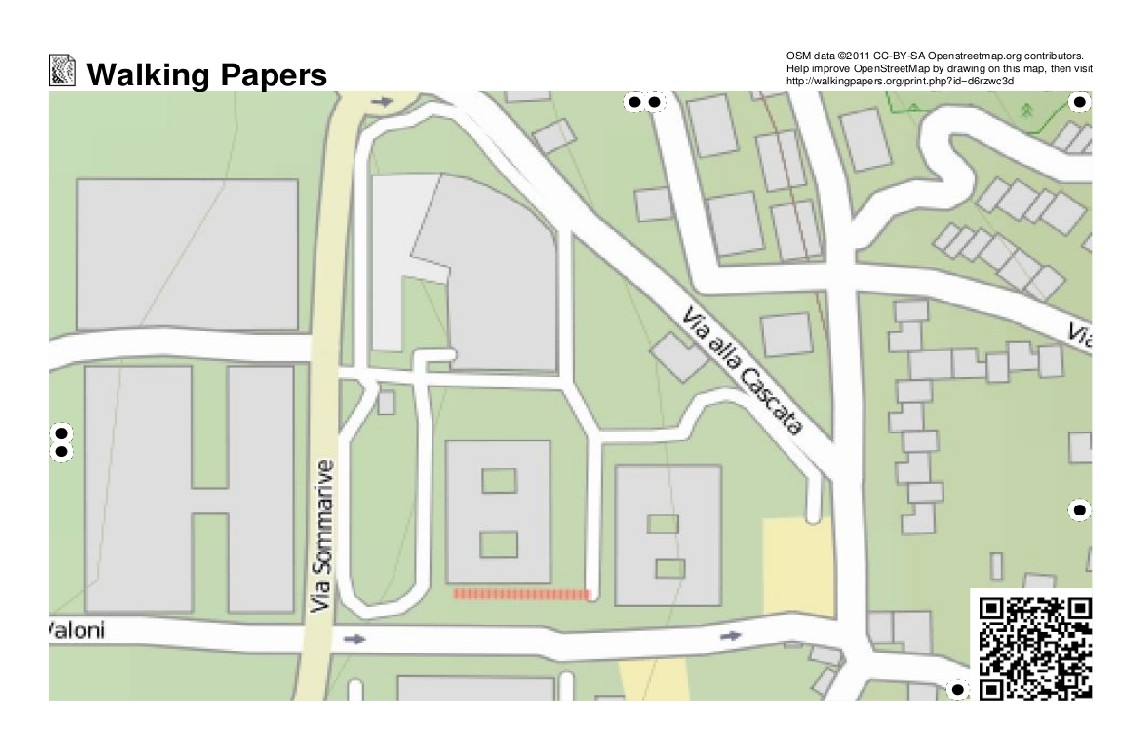
\includegraphics[width=1\textwidth]{../img/osm/walking}
		\end{center}
	\end{frame}

	% -----------------------------------------------------

	\begin{frame}
		\begin{columns}[c]
			\column{.4\textwidth}
				\begin{center}
					
\includegraphics[width=0.8\textwidth]{../img/archeo/question}
				\end{center}
			\column{.6\textwidth}
				\huge Cosa posso farci?
		\end{columns}
	\end{frame}

	% -----------------------------------------------------

	\begin{frame}{Fermata dell'autobus}{Košice, Slovacchia}
		\begin{center}
			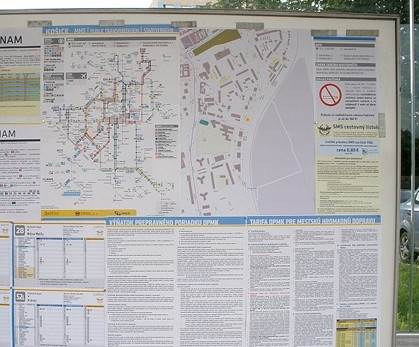
\includegraphics[width=0.8\textwidth]{../img/osm/bus}
		\end{center}
	\end{frame}

	% -----------------------------------------------------

	\begin{frame}{Calcolo percorsi}{www.openrouteservice.org -- University of Heidelberg}
		\begin{center}
			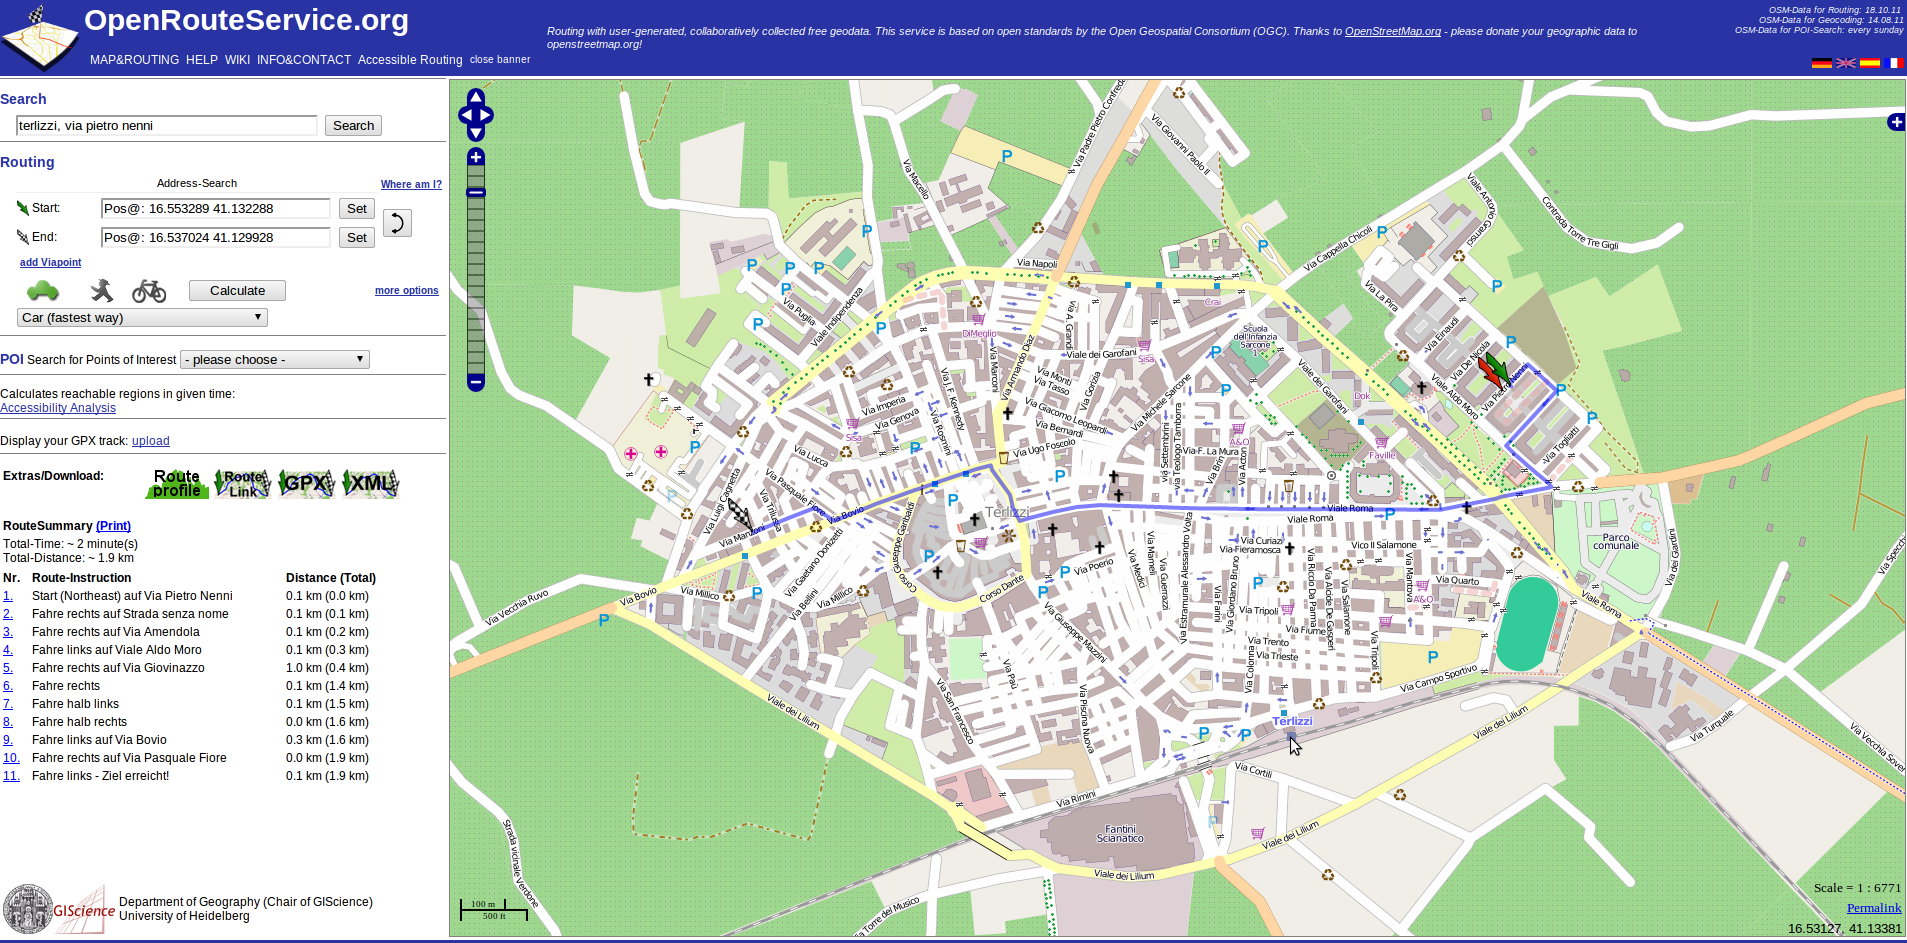
\includegraphics[width=1\textwidth]{../img/osm/openrouteservice}
		\end{center}
	\end{frame}

	% -----------------------------------------------------

	\begin{frame}{Navigatore satellitare}{http://wiki.openstreetmap.org/wiki/Gosmore}
		\begin{center}
			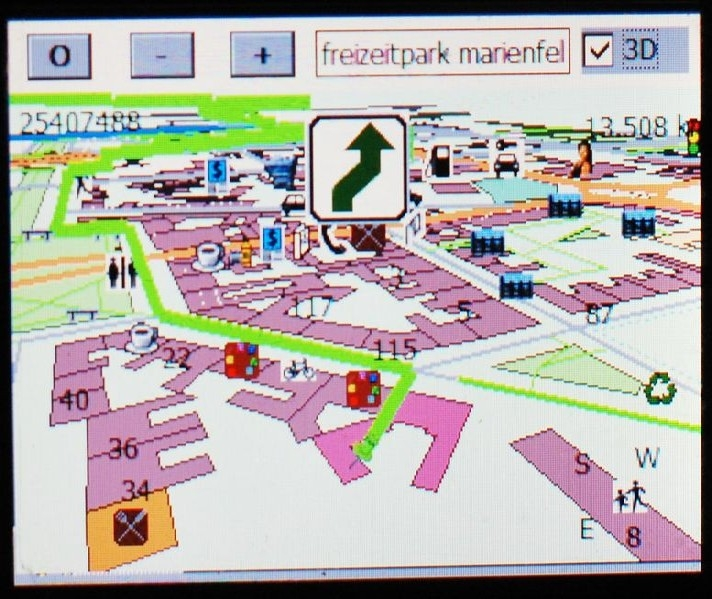
\includegraphics[width=0.8\textwidth]{../img/osm/gosmore}
		\end{center}
	\end{frame}

	% -----------------------------------------------------

	\begin{frame}{Usi creativi}{http://softcities.net}
		\begin{center}
			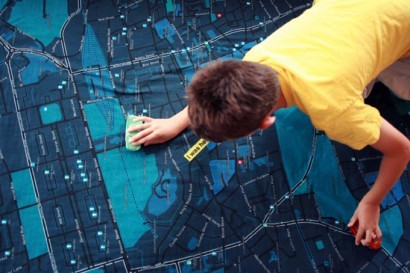
\includegraphics[width=0.8\textwidth]{../img/osm/blanket}
		\end{center}
	\end{frame}

	% -----------------------------------------------------

	\begin{frame}{\textit{Map of Copenhagen for young travellers}}{http://www.use-it.be/europe}
		\begin{center}
			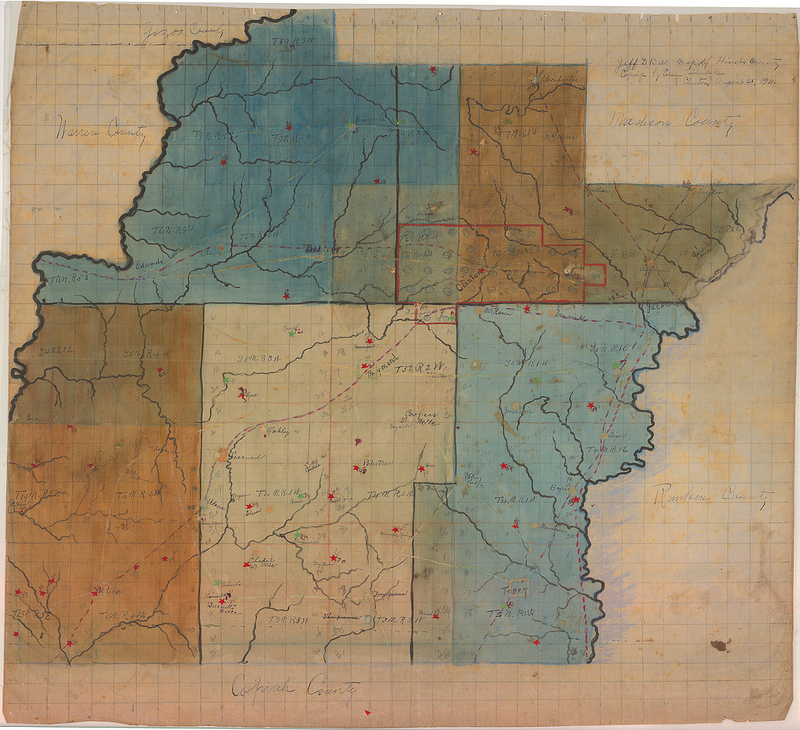
\includegraphics[width=0.8\textwidth]{../img/osm/map}
		\end{center}
	\end{frame}

	% -----------------------------------------------------

	\begin{frame}{Haiti earthquake -- prima}{Credits: http://www.flickr.com/photos/itoworld/4351891226}
		\begin{center}
			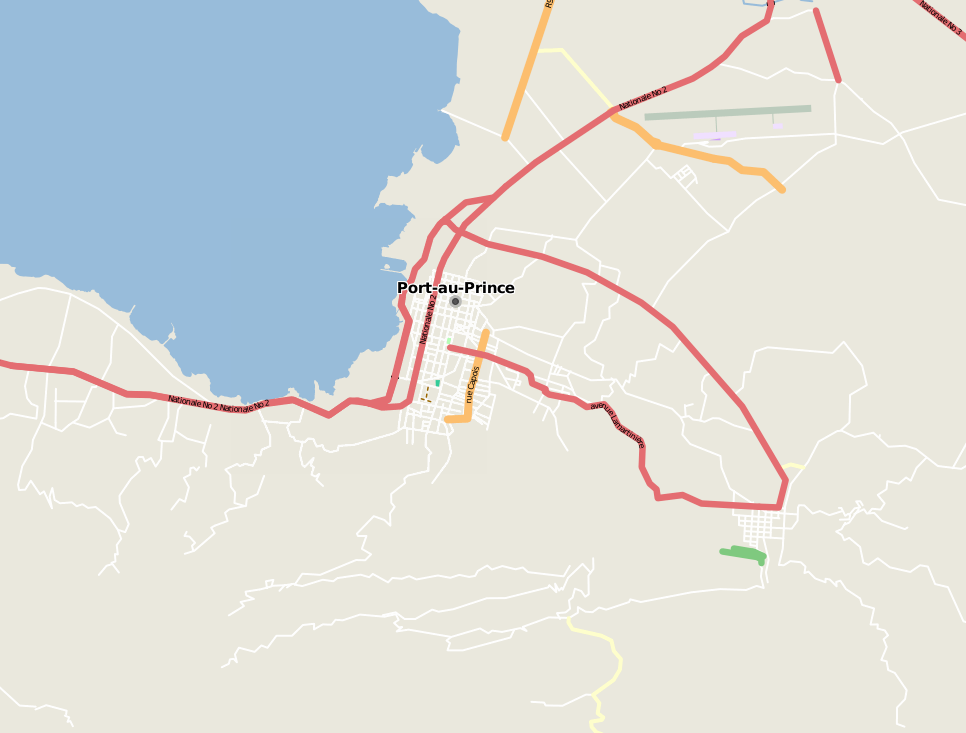
\includegraphics[width=0.9\textwidth]{../img/osm/haiti_pre}
		\end{center}
	\end{frame}

	% -----------------------------------------------------

	\begin{frame}{Haiti earthquake -- dopo}{Credits: http://www.flickr.com/photos/itoworld/4351891526}
		\begin{center}
			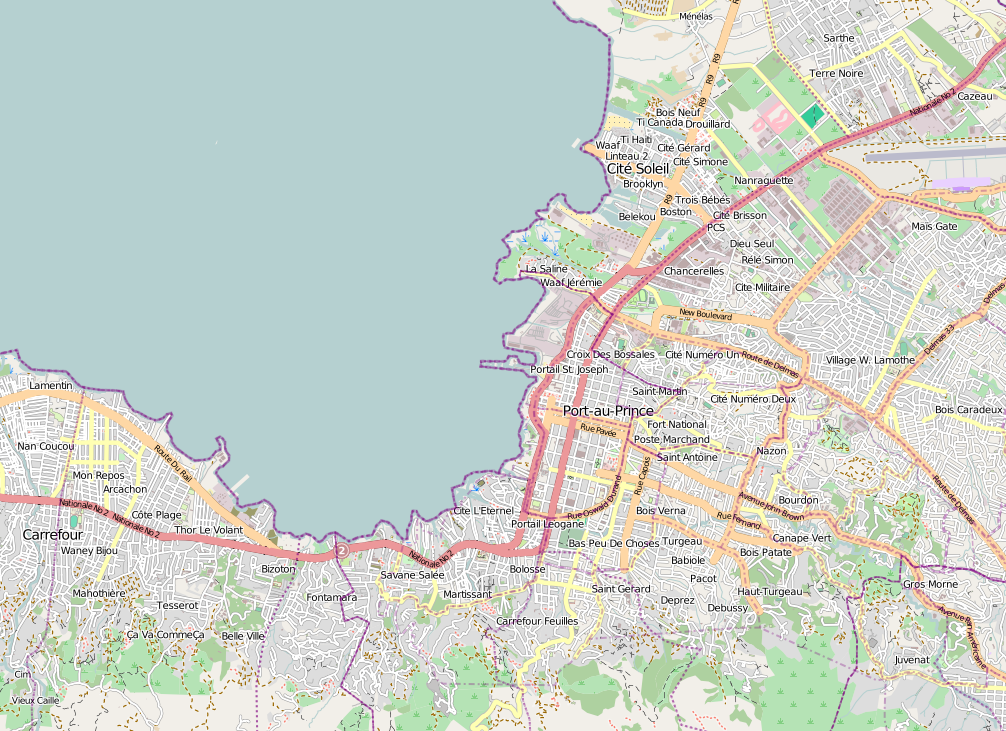
\includegraphics[width=0.9\textwidth]{../img/osm/haiti_post}
		\end{center}
	\end{frame}

	% -----------------------------------------------------

	\begin{frame}{Licenza}
		Tutti i geodati e le mappe di OpenStreetMap sono rilasciati con licenza

		\begin{center}
			\fontsize{50}{60}\selectfont \ccbysa
		\end{center}
		\begin{center}
			\textbf{Creative Commons}\\
			\textbf{Attribution -- Share Alike 2.0}
		\end{center}
	\end{frame}

	% -----------------------------------------------------

	\begin{frame}{Licenza}
		Tutti abbiamo le seguenti libertà:
		\begin{itemize}
			\item copiare e distribuire le mappe
			\item modifiare le mappe
			\item distribuire le versioni modifiate
			\item utilizzare per scopi commerciali le mappe
		\end{itemize}

		Purchè:
		\begin{enumerate}
			\item sia citata la fonte dei dati (OpenStreetMap)
			\item qualunque creazione derivata deve essere rilasciata sotto la stessa licenza
		\end{enumerate}
	\end{frame}

	% -----------------------------------------------------

	\begin{frame}{OpenStreetMap in breve}
		\begin{center}
			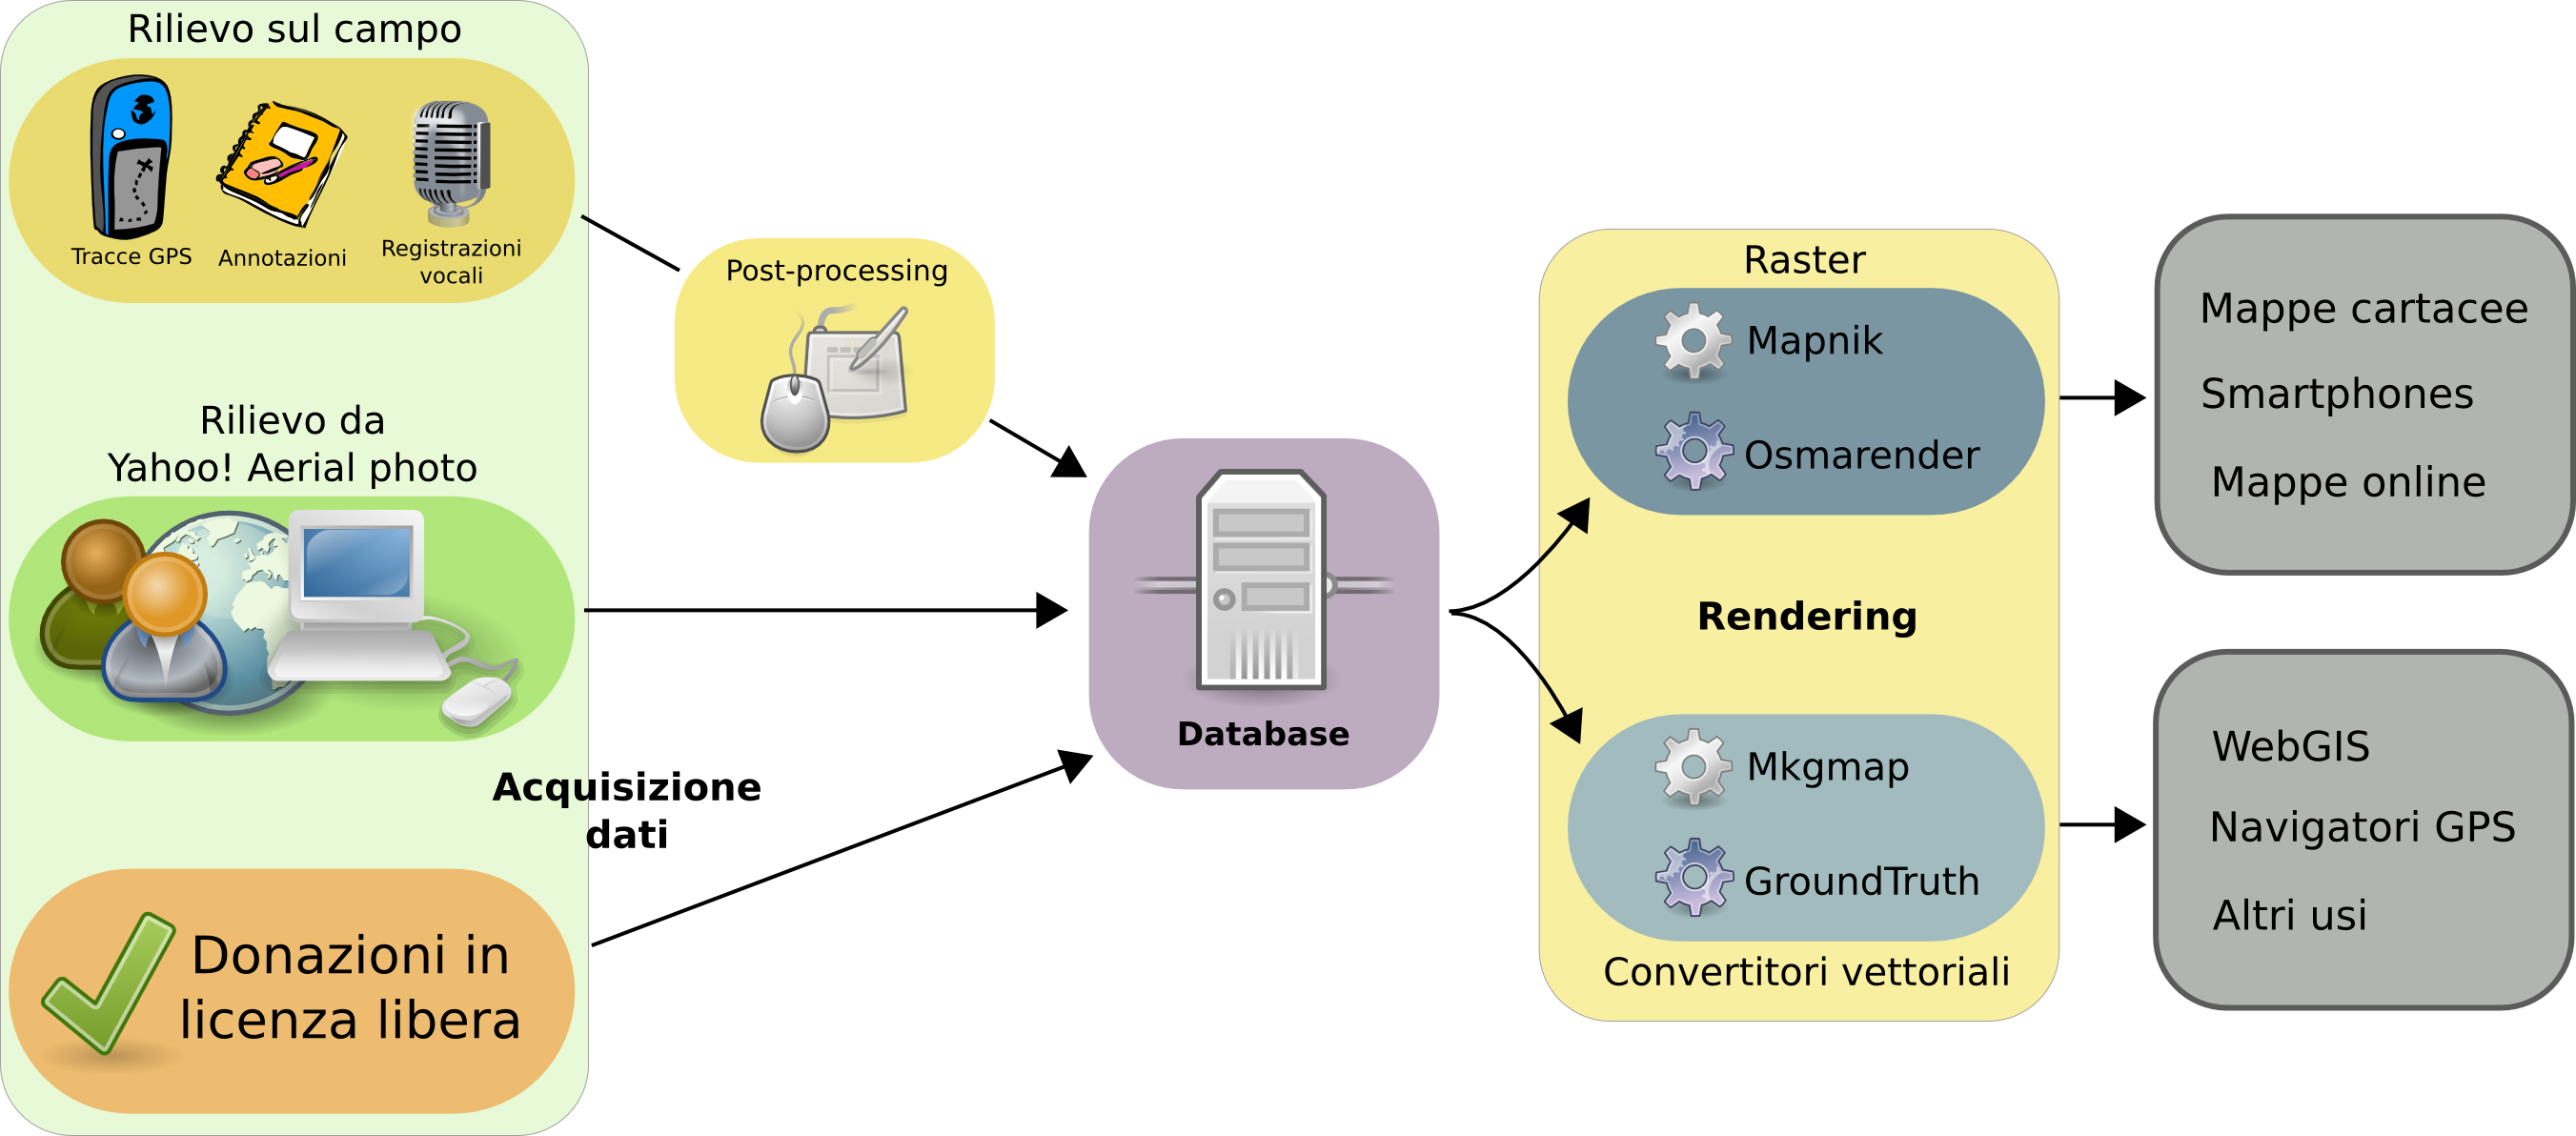
\includegraphics[width=1\textwidth]{../img/osm/osm_scheme}
		\end{center}
	\end{frame}

	% -----------------------------------------------------

	\begin{frame}{OpenStreetMap ed i beni culturali}{Punti d'interesse}
		Punti d'interesse (POI) che è possibile scaricare dal database di OSM:
		\begin{itemize}
			\item torri / castelli
			\item chiese
			\item cappelle votive
			\item croci a bordo strada
			\item rovine
			\item scavi archeologici
			\item musei
			\item punti d'interesse turistico generici
			\item belvedere
			\item lapidi / memoriali
			\item naufragi / relitti
			\item campi di battaglia
			\item opere d'arte all'aperto / monumenti
		\end{itemize}
	\end{frame}

	% -----------------------------------------------------

	\begin{frame}{2008: OSM mappa Pompei}{07--12--2008}
		\begin{center}
			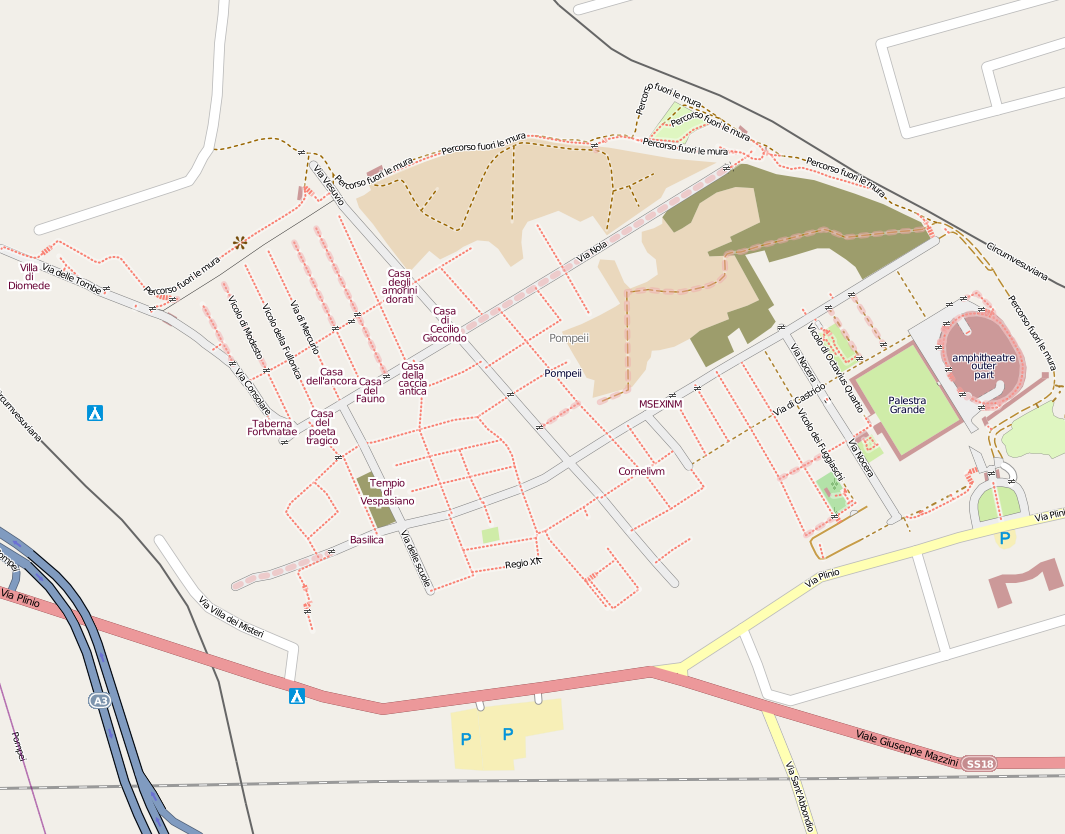
\includegraphics[width=0.9\textwidth]{../img/osm/pompeii}
		\end{center}
	\end{frame}

	% -----------------------------------------------------
	% -----------------------------------------------------

	\begin{frame}{~}
		\begin{center}
			\huge
			Now for something\\completely different
		\end{center}
		\vfill
		\begin{flushright}
			\Large \ldots ma non troppo.
		\end{flushright}
	\end{frame}

	% -----------------------------------------------------
	% -----------------------------------------------------
\end{document}
